\section{Gdev Ecosystem}
\label{sec:ecosystem}

\begin{figure}[t]
 \begin{center}
  %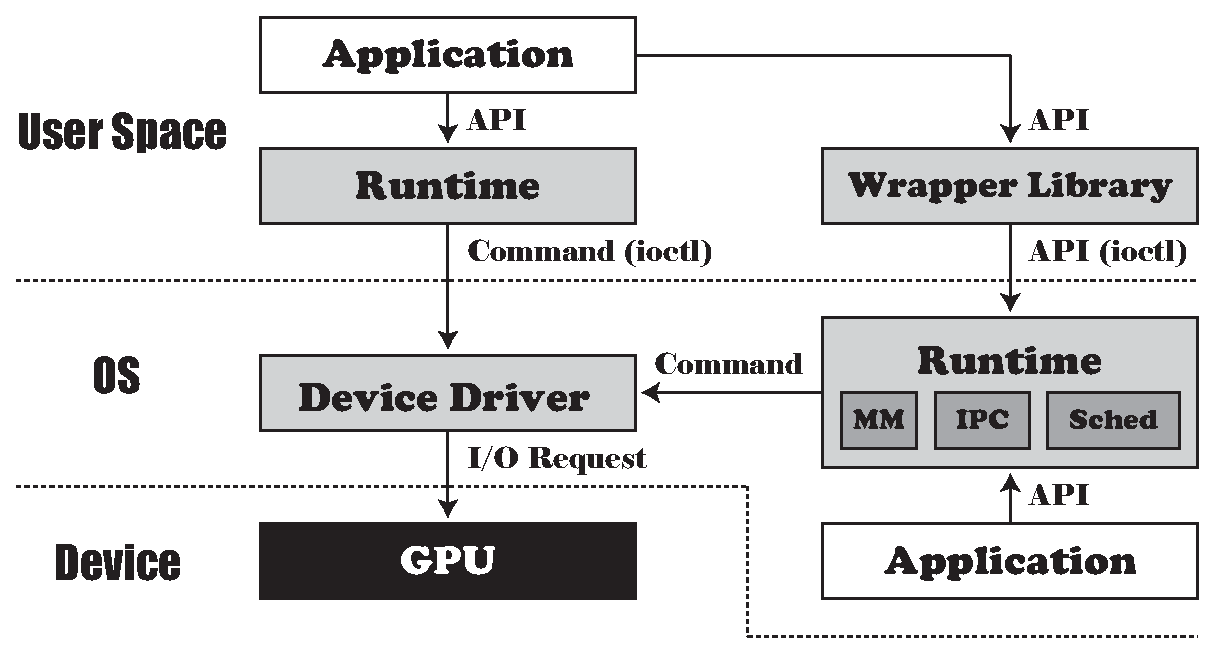
\includegraphics[width=\hsize]{eps/gdev.eps}\\
  \caption{Logical view of Gdev ecosystem.}
  \label{fig:gdev}
 \end{center}
 \vspace{-1em}
\end{figure}

Gdev is aimed at extending GPU resource management capabilities and a
class of applications that can benefit from the GPU.
To this end, it integrates runtime support into the OS.
Figure~\ref{fig:gdev} illustrates the overview of the Gdev ecosystem.
First of all, Gdev still supports a traditional execution model, where
applications call the user-space runtime library through the API, and
the library sends a series of GPU commands to the device driver through
the system call.
As demonstrated in previous work~\cite{Kato_ATC11}, however, it is hard
to analyze what the sequence of GPU commands means at runtime by
software (there could be hundreds of commands for one operation).
It would not therefore be appropriate to call resource management
primitives along with command calls but with API calls.
This argument motives the Gdev design below.

Unlike traditional approaches, Gdev employs runtime support in
the OS, providing GPU resource management primitives along with the API.
OS applications can use this runtime directly, while user-space
applications can also use it through the wrapper library provided by
Gdev, which simply relays API calls to the OS runtime using the system
call.
This runtime-unified approach enables Gdev to be API-driven, where the
scheduler, for instance, is invoked for GPU computations and host-device
data transmissions upon corresponding API calls.

\begin{table}[t]
 \caption{Representatives of Gdev API.}
 \label{tab:gdev_api}
 \begin{center}
  {\small
  \begin{tabular}{|l|l|}
   \hline
   \textbf{API name} & \textbf{Description}\\
   \hline
   \texttt{gopen}/\texttt{gclose} & Open/close the device\\
   \hline
   \texttt{gmalloc}/\texttt{gfree} & Allocate/free device memory\\
   \hline
   \texttt{gmalloc\_io}/\texttt{gfree\_io} & Allocate/free host I/O memory\\
   \hline
   \texttt{gmemcpy\_to\_device} & Copy memory to the device\\
   \hline
   \texttt{gmemcpy\_from\_device} & Copy memory from the device\\
   \hline
   \texttt{gmemcpy\_in\_device} & Copy memory within the device\\
   \hline
   \texttt{glaunch}/\texttt{gsync} & Launch/wait computation\\
   \hline
   \texttt{gquery} & Query device information\\
   \hline
   \texttt{gshmget}/\texttt{gshmctl} & Manage shared device memory\\
   \hline
   \texttt{gshmat}/\texttt{gshmdt} & Share/unshare device memory\\
   \hline
  \end{tabular}
  }
 \end{center}
\vspace{-1em}
\end{table}

\textbf{Low-Level API:}
Gdev provides a set of low-level API functions for GPU programming as
shown in Table~\ref{tab:gdev_api}.
Programmers can use either the Gdev API or a high-level API, such as
CUDA, which is built on top of the Gdev API.
In either case, Gdev API is eventually used to access the GPU.
There are several more API functions supported by Gdev, such as
asynchronous memory copy functions, but are not focused on in this
paper.

Table~\ref{tab:gdev_api} shows an initial version of Gdev API.
For now, Gdev API does not support texture memory and 2-D/3-D memory
transfers.
Although this is a current limitation on our prototype implementation,
it is not a conceptual limitation of Gdev.
We believe that the Gdev resource management presented in this paper is
also applicable to those extensions once the API is supported.

\textbf{CUDA Support:}
In addition to Gdev API, we provide CUDA 4.0 Driver API~\cite{CUDA40}
support so that legacy CUDA applications can run on top of Gdev in both
the user space and OS.
The supported API functions are limited to those that can be implemented
by the current version of Gdev API, but many legacy CUDA applications
can perform with this limited set of API, as we will show in
Section~\ref{sec:evaluation}.

Gdev assumes that programs are compiled by NVIDIA CUDA Compiler
(NVCC)~\cite{CUDA40}.
Since CUDA Driver API separates device binary and host binary, Gdev only
needs to parse the device binary to aquire static information, such
as the code size, stack size, shared memory size, local memory size, and
parameters size, when it is loaded by the host binary.
Global memory is also dynamically allocated by the host binary at
runtime.
It should be noted that CUDA also provides a different type of API,
called Runtime API, which is more high-level than Driver API.
Although the current implementation of Gdev does not support CUDA
Runtime API by itself, we could leverage Ocelot~\cite{Diamos_PACT10} to
translate Runtime API to Driver API, in order to run CUDA programs
written in Runtime API.

\textbf{First-Class Resource Management:}
Gdev supports first-class memory management and scheduling for the GPU
to allow time-sharing multi-tasking systems to use the GPU
efficiently.
Our Gdev approach classifies GPU resource management primitives into
the device, virtual address space, context, and memory objects,
abstracted for a generalization of our approach.